\documentclass[a4paper]{scrreprt}

\usepackage[ngerman]{babel}
\usepackage[utf8]{inputenc}
\usepackage[T1]{fontenc}
\usepackage{ae}
\usepackage[bookmarks, bookmarksnumbered]{hyperref}
\usepackage{tabularx}
\usepackage{graphicx}
\usepackage{csquotes}
\usepackage{verbatim}
\usepackage[nonumberlist, toc, section]{glossaries}
\usepackage[german]{fancyref}

\makeglossaries

\setcounter{secnumdepth}{3}


% Document
% zu jedem umgesetzten Punkt des Pflichtenhefts Bezug herstellen

\begin{document}

    \tableofcontents
    \chapter{Einleitung}
    \chapter{Architekturdiagramm}

    \chapter{Klassendiagramme}
    \section{API}
    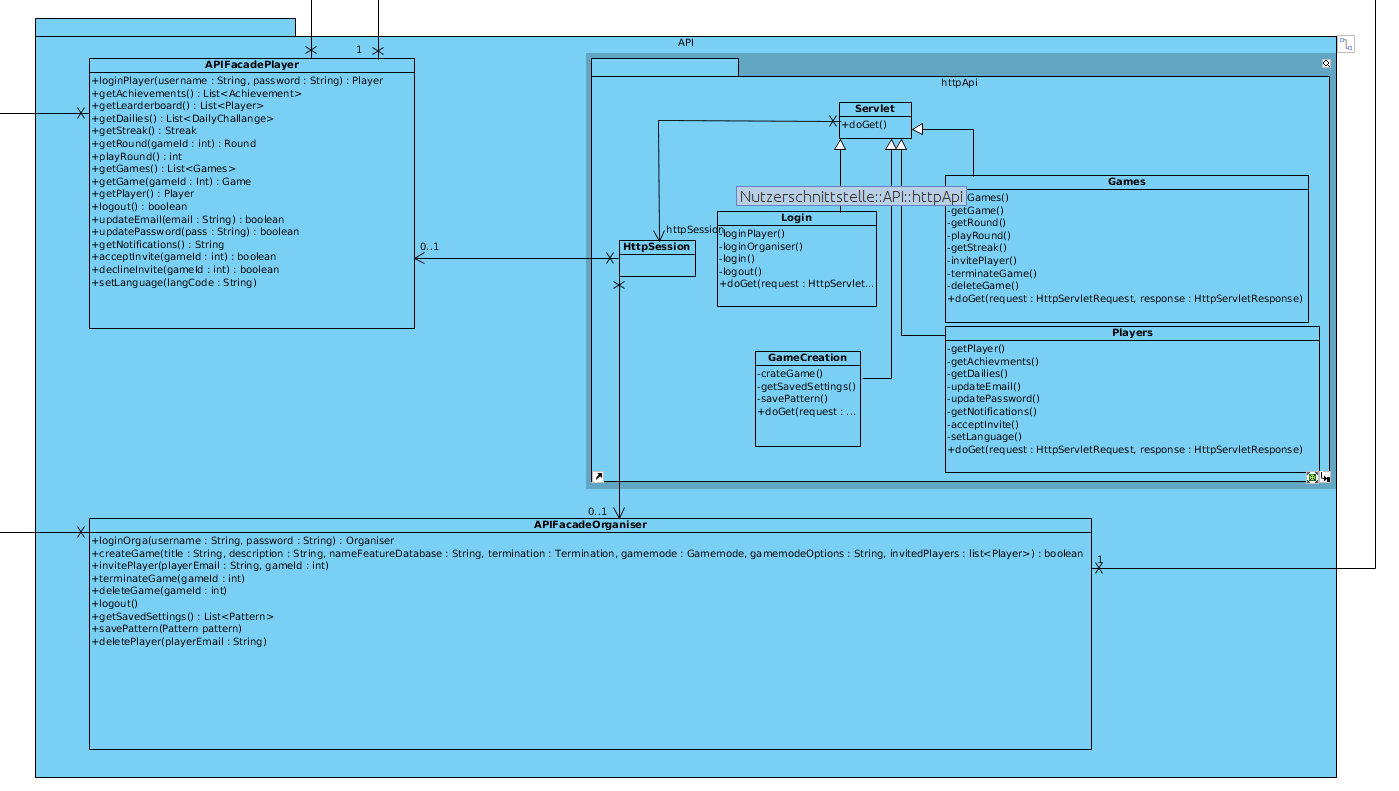
\includegraphics[width=\textwidth]{img/api.png}
    \subsection{APIFacadePlayer}
        Eine APIFacadePlayer ist das Objekt, über welches sämtliche Interaktion mit dem System von den Spielern aus passiert. Nach dem Konstruktor \textbf{muss} zuerst loginPlayer aufgerufen werden, bis es erfolgreich zurückkehrt. Ansonsten haben alle anderen Methoden kein definiertes Verhalten und werden im Allgemeinem nichts nützliches zurückgeben. Eine APIFacadePlayer ist immer mit einem Spieler assoziert, falls dieser korrekt angemeldet wurde. Alle Methoden beziehen sich dann auf den angemeldeten Spieler.
    \subsubsection{loginPlayer}
        \begin{itemize}
            \item Beschreibung: Versucht einen Spieler mit email und password anzumelden. Bei Erfolg wird diese Facade mit dem Spieler assoziert.
            \item Parameters: 
                \begin{itemize}
                    \item email: Die Email Adresse mit der eine Anmeldung versucht wird
                    \item password: Das Passwort zu mit dem eine Anmeldung versucht wird
                \end{itemize}
            \item Rückgabewert: Falls die Email-Passwort Kombination einen validen Spieler beschreibt, wird dieser zurückgegeben. Andernfalls wird null zurückgegeben.
        \end{itemize}
    \subsubsection{logout}
    \begin{itemize}
        \item Beschreibung: Meldet den angemeldeten Spieler ab. Nach dem Aufruf dieser Methode verhält sich dieses Objekt wieder so, als ob nie ein Spieler angemeldet wurde
    \end{itemize}
    \subsubsection{getAchievments}
    \begin{itemize}
        \item Beschreibung: Holt die Liste aller Achievments, mit der Information ob der Spieler diese bereits erreicht hat oder nicht.
        \item Rückgabewert: Liste an Achievments. 
    \end{itemize}
    \subsubsection{getLeaderboard}
    \begin{itemize}
        \item Beschreibung: Gibt das aktuelle Leaderboard in der geordneten Reihenfolge zurück
        \item Rückgabewert: Eine Liste an Spielern, geordnet nach ihrer Leaderboard-Ordunung. 
    \end{itemize}
    \subsubsection{getDailies}
    \begin{itemize}
        \item Beschreibung: Gibt die Daily-Challenges für diesen Spieler zurück, mit der Information, wie weit diese bereits erfüllt sind.
        \item Rückgabewert: Eine Liste an Daily-Challenges für diesen Spieler mit Information, wie weit diese erfüllt sind.
    \end{itemize}
    \subsubsection{getStreak}
    \begin{itemize}
        \item Beschreibung: Gibt das aktuelle Streak-Objekt für diesen Spieler zurück
        \item Rückgabewert: Das aktuelle Streak-Objekt für diesen Spieler 
    \end{itemize}
    \subsubsection{getPoints}
    \begin{itemize}
        \item Beschreibung: Gibt die Punkte des Spielers zurück
        \item Rückgabewert: Aktuelle Punktzahl des Spielers 
    \end{itemize}
    \subsubsection{getRound}
    \begin{itemize}
        \item Beschreibung: Fordert die nächste Runde für ein Spiel an und gibt diese zurück
        \item Parameter:
        \begin{itemize}
            \item gameId: Eindeutige Id des Spieles für das die Runde angefordert wird
        \end{itemize}
        \item Rückgabewert: Wenn der Spieler eine Runde in dem angegebenem Spiel spielen darf, dann wird das Runden-Objekt zurückgegen. Andernfalls wird null zurückgegeben 
    \end{itemize}
    \subsubsection{playRound}
    \begin{itemize}
        \item Beschreibung: Spielt eine Runde in der aktuellen Runde
    \end{itemize}
    \subsubsection{getGames}
    \begin{itemize}
        \item Beschreibung: Holt alle Spiele, an denen der Spieler teilnimmt
        \item Rückgabewert: Liste an Spielen, an denen der Spieler teilnimmt 
    \end{itemize}
    \subsubsection{getGame}
    \begin{itemize}
        \item Beschreibung: Gibt ein Spiel nach Id zurück, falls der Spieler auf dieses Spiel Zugriff hat
        \item Parameter:
        \begin{itemize}
            \item gameId: die Id des Spiels, welches zurückgegeben werden soll
        \end{itemize}
        \item Rückgabewert: Falls gameId valid ist, also Spiel existiert und Spieler darf auf das Spiel zugreifen, dann wird das Spiel zurückgegen, ansonsten null. 
    \end{itemize}
    \subsubsection{getPlayer}
    \begin{itemize}
        \item Beschreibung: Gibt den angemeldeten Spieler zurück. Also der Spieler, welcher durch loginPlayer angemeldet wurde.
        \item Rückgabewert: Der angemeldete Spieler, falls keiner angemeldet ist wird null zurückgegeben. 
    \end{itemize}
    \subsubsection{updateEmail}
    \begin{itemize}
        \item Beschreibung: Ändert die E-Mail-Adresse mit der sich ein Spieler anmeldet. Die Änderung tritt erst in Effekt, wenn die neue Email-Adresse bestätigt wurde.
        \item Parameter:
        \begin{itemize}
            \item email: Die neue E-Mail-Adresse, welche in Zukunft für diesen Spieler verwendet werden soll.
        \end{itemize}
        \item Rückgabewert: true falls die Bestätigungsemail veschickt wurde, false andernfalls 
    \end{itemize}
    \subsubsection{updatePassword}
    \begin{itemize}
        \item Beschreibung: Ändert das Passwort mit dem sich der Spieler anmeldet. Die Änderung tritt sofort in Effekt.
        \item Parameter:
        \begin{itemize}
            \item pass: Das neue Passwort
        \end{itemize}
        \item Rückgabewert: true falls die Änderung erfolgreich war, false andernfalls 
    \end{itemize}
    \subsubsection{getNotifications}
    \begin{itemize}
        \item Beschreibung: Holt alle Notifications, die für diesen Spieler anliegen
        \item Rückgabewert:  Alle Notifications, die für diesen Spieler anliegen
    \end{itemize}
    \subsubsection{acceptInvite}
    \begin{itemize}
        \item Beschreibung: Akzeptiert eine Einladung zu einem Spiel, welche diesem Spieler geschickt wurde und löscht diese aus seinen Einladungen
        \item Parameter:
        \begin{itemize}
            \item gameId: Id des Spiels für das die Einladung angenommen werden soll.
        \end{itemize}
        \item Rückgabewert: true wenn die Einladung angenommen wurde, false falls der Spieler keine Einladung zu diesem Spiel hatte, das Spiel nicht existier oder bereits beendet ist. 
    \end{itemize}
    \subsubsection{declineInvite}
    \begin{itemize}
        \item Beschreibung: Lehnt eine Einladung zu einem Spiel ab, welche diesem Spieler geschickt wurde und löscht diese aus seinen Einladungen
        \item Parameter:
        \begin{itemize}
            \item gameId: Id des Spiels für das die Einladung abgelehnt werden soll.
        \end{itemize}
        \item Rückgabewert: true wenn die Einladung abgelehnt wurde, false falls der Spieler keine Einladung zu diesem Spiel hatte, das Spiel nicht existier oder bereits beendet ist. 
    \end{itemize}
    \subsubsection{setLanguage}
    \begin{itemize}
        \item Beschreibung: Setzt die Sprache für den Spieler
        \item Parameter:
        \begin{itemize}
            \item langCode: der Landescode für die gewünschte Sprache
        \end{itemize}
    \end{itemize}
    \subsection{APIFacadeOrganiser}
    \subsubsection{loginOrganiser}
    \begin{itemize}
        \item Beschreibung: meldet einen Organisator an. Damit dies möglich ist, muss der Organisator vorher registriert worden sein.
        \item Parameter:
        \begin{itemize}
            \item email: E-Mail des anzumeldenden Organisators
            \item password: Das Passwort des anzumeldenden Organisators
        \end{itemize}
        \item Rückgabewert: Falls die Email-Passwort Kombinnation valid ist, also ein Organisator mit der E-Mail registriert ist und das Passwort ist richtig, wird der Organisator zurückgegeben. Andernfalls null. 
    \end{itemize}
    \subsubsection{createGame}
    \begin{itemize}
        \item Beschreibung: erstellt ein Spiel für diesen Organisator.
        \item Parameter: %% stuff bleibt hier ja noch nicht ganz fest gegeben
        \begin{itemize}
            \item :
        \end{itemize}
        \item Rückgabewert: Falls das Erstellen erfolgreich war, true zurückgegeben, andernfalls false. 
    \end{itemize}
    \subsubsection{invitePlayer}
    \begin{itemize}
        \item Beschreibung: Lädt einen Spieler zu einem Spiel des Organisators ein.
        \item Parameter:
        \begin{itemize}
            \item playerEmail: die Email-Adresse des einzuladenden Spielers
            \item gameId: Das Spiel, zu dem der Spieler eingeladen werden soll. Das Spiel muss ein Spiel des Organisators sein.
        \end{itemize}
    \end{itemize}
    \subsubsection{terminateGame}
    \begin{itemize}
        \item Beschreibung: Beendet ein Spiel des Organisators. 
        \item Parameter:
        \begin{itemize}
            \item gameId: Id des zu beendenden Spiels. Das Spiel muss zu dem Organisator gehören.
        \end{itemize}
    \end{itemize}
    \subsubsection{deleteGame}
    \begin{itemize}
        \item Beschreibung: Löscht ein Spiel des Organisators aus dem System. 
        \item Parameter:
        \begin{itemize}
            \item gameId: Die Id des zu löschende Spiel
        \end{itemize}
    \end{itemize}
    \subsubsection{logout}
    \begin{itemize}
        \item Beschreibung: Meldet einen Organisator ab. Nach dem Aufruf dieser Methode verhält sich dieses Objekt so, als ob niemand angemeldet war.
    \end{itemize}
    \subsubsection{getSavedSettings}
    \begin{itemize}
        \item Beschreibung: Holt eine Liste aller gespeicherten Einstellungen dieses Organisators.
        \item Rückgabewert: Eine Liste aller gespeichterten Einstellungen dieses Organisators. 
    \end{itemize}
    \subsubsection{savePattern}
    \begin{itemize}
        \item Beschreibung: Speichert eine Einstellungskonfiguration für diesen Organisator
        \item Parameter:
        \begin{itemize}
            \item pattern: Das zu speichernde Pattern
        \end{itemize}
    \end{itemize}

    \section{Database}
    \subsection{DatabaseAdapter}
    \subsection{UserAdapter}
    \subsection{PlayerAdapter}
    \subsection{OrganiserAdapter}
    \subsection{GameAdapter}
    \subsection{Mysql}
    \subsubsection{MysqlDatabaseAdapter}
    \subsubsection{MysqlUserAdapter}
    \subsubsection{MysqlPlayerAdapter}
    \subsubsection{MysqlOrganiserAdapter}
    \subsubsection{MysqlGameAdapter}

    \section{MLServer}
    \subsection{MLServer}
    \subsection{RESTMLServer}

   \chapter{Sequenzdiagramme}

    \chapter{Datenhaltung}
        \section{Ordnerstruktur}
        \section{Konfiguration}
        \section{Datenbank}



\end{document}
